%    Copyright 2017 Marc Demierre, HES-SO//Master
%
% Licensed under the Apache License, Version 2.0 (the "License");
% you may not use this file except in compliance with the License.
% You may obtain a copy of the License at
%
% http://www.apache.org/licenses/LICENSE-2.0
%
% Unless required by applicable law or agreed to in writing, software
% distributed under the License is distributed on an "AS IS" BASIS,
% WITHOUT WARRANTIES OR CONDITIONS OF ANY KIND, either express or implied.
% See the License for the specific language governing permissions and
% limitations under the License.

% =============================================================================
% | HES-SO//Master - Thesis project report template                           |
% |                                                                           |
% | Originally based on the EPFL template, with many adjustements             |
% =============================================================================

% Document settings
\documentclass[a4paper,11pt,fleqn]{book}
\usepackage[utf8]{inputenc}
\usepackage[T1]{fontenc}
\usepackage[french,english]{babel}

% -----------------------------------------------------------------------------
% Preamble
% -----------------------------------------------------------------------------
% =============================================================================
% | Thesis metadata                                                           |
% =============================================================================

% Thesis info
\newcommand{\ThesisTitle}{Création de composants BI custom dans Power BI}
\newcommand{\ThesisSubject}{[ThesisSubject]}
\newcommand{\Orientation}{Information and Communication Technologies (ICT)}
\newcommand{\Keywords}{keyword1, keyword2, keyword3}

% Author
\newcommand{\AuthorFirstName}{Blendar}
\newcommand{\AuthorLastName}{Berisha}
\newcommand{\AuthorEmail}{blendar.berisha@students.hevs.ch}
\newcommand{\Author}{\AuthorFirstName\ \AuthorLastName}

% Advisor
\newcommand{\AdvisorFirstName}{Cosette}
\newcommand{\AdvisorLastName}{Bioley}
\newcommand{\AdvisorSchool}{HES-SO Valais-Wallis}
\newcommand{\Advisor}{Prof. \AdvisorFirstName\ \AdvisorLastName}

% Place (for date and place)
\newcommand{\Date}{\today}
\newcommand{\Place}{Sierre}

\newcommand{\SubmissionDate}{14 août 2025}
         % your project data
% ==================
% Template settings
% ==================

% General tools
% -------------
\usepackage{etoolbox}

% Page style
% ----------
\usepackage[margin=2.5cm, left=2.5cm, right=2.5cm, twoside=true]{geometry}
\usepackage{fancyhdr}
\setlength{\headheight}{14pt}
\renewcommand{\sectionmark}[1]{\markright{\thesection\ #1}}
\pagestyle{fancy}

% Standard pages (inside chapters)
\fancyhf{}
\renewcommand{\headrulewidth}{0.4pt}
\renewcommand{\footrulewidth}{0pt}
\fancyhead[OR]{\bfseries \nouppercase{\rightmark}}
\fancyhead[EL]{\bfseries \nouppercase{\leftmark}}
\fancyfoot[EL,OR]{\thepage}

% First page of chapters
\fancypagestyle{plain}{
	\fancyhf{}
	\renewcommand{\headrulewidth}{0pt}
	\renewcommand{\footrulewidth}{0pt}
	\fancyfoot[EL,OR]{\thepage}
}

% Imports for external PDFs
\fancypagestyle{addpagenumbersforpdfimports}{
	\fancyhead{}
	\renewcommand{\headrulewidth}{0pt}
	\fancyfoot{}
	\fancyfoot[RO,LE]{\thepage}
}

% Use empty style for page when clearing double pages
\def\cleartoodd{%
	\clearpage%
%	\ifodd\value{page}\else\mbox{}\thispagestyle{empty}\newpage\fi%
}

%\def\clearchap{%
%	\ifodd\value{page}\else\mbox{}\thispagestyle{empty}\fi%%
%}

% \cleardoublepage replaced by \cleartoodd
\let\origdoublepage\cleardoublepage
\renewcommand{\cleardoublepage}{%
	\cleartoodd%
}

% Fonts
% -----

% Helvetica (Arial used in the MSE Word template)
\usepackage{helvet}

% Math
% ----
\usepackage{amsmath}  % better math

% Floats and figures
% ------------------
\usepackage{newfloat}          % floats
\usepackage[twoside]{caption}  % captions
\usepackage{subcaption}        % subcaptions
\usepackage[section]{placeins} % allows to put float barriers

% Float captions in italics, with label in margin
\DeclareCaptionLabelFormat{title}{#1 #2}
\DeclareCaptionLabelFormat{hangout}{\llap{#1 #2\hspace{0.3em}}}
\captionsetup{
    justification=centering,
	% format=hang,
	% labelformat=hangout,
	singlelinecheck=on,
	font={it},
	% labelsep = colon
}

% Caption with source for figure
% TODO: improve this to use square brackets like the normal "caption"
\newcommand*{\captionsource}[3]{%
	\caption[{#1}]{%
		#2%
		
		\textbf{Source:} #3%
	}%
}

% Tables
% ------
\usepackage{booktabs} % much better tables
\usepackage{multirow} % allows to fuse rows
\usepackage{array}    % manipulate array
\usepackage{tabularx} % better tables

% Define new tabularx column types:
%  - R: streteched right aligned
%  - C: stretched centered
%  - N: left aligned, specified space
\newcolumntype{R}{>{\raggedleft\arraybackslash}X}%
\newcolumntype{C}{>{\centering\arraybackslash}X}%
\newcolumntype{N}[1]{>{\raggedleft\arraybackslash}p{#1}}

% Set row height multiplicator to provide more breathing space
\renewcommand{\arraystretch}{1.3} 

% Bibliography
% -------------------

% Use APA style
\usepackage[backend=biber, style=apa6]{biblatex}
\DeclareLanguageMapping{french}{french-apa}
\addbibresource{03-tail/bibliography.bib}
\DefineBibliographyStrings{french}{
  nodate    = {{}s.\adddot\addspace d\adddot},
}

% Tables of contents, figures, tables and listings
% ------------------------------------------------
\usepackage{tocloft}
\newlistof{listing}{lol}{List of Listings}
\setcounter{tocdepth}{1} % Depth to 'section'
\setlength{\cftfigindent}{0pt}  % remove indentation from figures in lof
\setlength{\cftfignumwidth}{1cm}
\setlength{\cfttabindent}{0pt}  % remove indentation from tables in lot
\setlength{\cfttabnumwidth}{1cm}
\setlength{\cftlistingindent}{0pt}
\setlength{\cftlistingnumwidth}{1cm}

% Mini tables of contents
% -----------------------
\usepackage{minitoc}

% no "Contents" title
\mtcsettitle{minitoc}{Contents} 

% Layout
\setlength{\mtcindent}{-0.5em}
\mtcsetoffset{minitoc}{-1em}

% Spacing above and below table
\mtcsetfeature{minitoc}{before}{\vspace{0.5cm}}
\mtcsetfeature{minitoc}{after}{\vspace{-0.25cm}}
\renewcommand{\mtifont}{\sffamily\bfseries\large}

% Colors & graphics
% -----------------
\usepackage[table]{xcolor}    % colors
\usepackage[pdftex]{graphicx} % graphics importing
\graphicspath{{02-main/figures/}}
\definecolor{gray80}{gray}{0.80}


% Code and syntax highlighting
% ----------------------------
\usepackage[newfloat]{minted}   % code highlighting

% Typography
% ----------
\usepackage{csquotes}                    % paragraph indentation and spacing
\usepackage[defaultlines=3,all]{nowidow} % avoid widows and orphans
\usepackage{microtype}                   % typographic improvements
\usepackage{parskip}                     % No indent and auto-space between paragraphs
\usepackage[super]{nth}

\usepackage{paralist}
\usepackage{enumitem}
\setlist{after=\vspace{\baselineskip}}

% Section and chapters headings
% -----------------------------
\usepackage[explicit]{titlesec} % titles formatting
%\usepackage{titletoc} % titles formatting in ToC etc
%\usepackage{sectsty}  % sectioning commands

% -- Chapters --
% Remove "Chapter N" and use a sans-serif font

% Set layout lengths
\setlength{\headheight}{8mm}
\setlength{\footskip}{1.5cm}
\addtolength{\textheight}{-.5cm}

\titlespacing{\chapter}{0mm}{-10mm}{3mm}
\titlespacing{\section}{0mm}{11pt}{11pt}
\titlespacing{\subsection}{0mm}{11pt}{11pt}
\titlespacing{\subsubsection}{0mm}{11pt}{11pt}


%\titleformat{\chapter}[block]
%{\Huge}
%{\thechapter\hspace{12pt}\textcolor{gray80}{|}\hspace{12pt}}
%{0pt}
%{\Huge\bfseries}

\titleformat{\chapter}{\Huge\bfseries}{\thechapter\hspace{12pt}\textcolor{gray80}{|}}{5mm}{%
	\hfill\begin{minipage}[t]{\dimexpr\textwidth}\raggedright#1\end{minipage}%
}
\titleformat{\section}{\Large\bfseries}{\thesection}{0.7em}{%
	\begin{minipage}[t]{\dimexpr\textwidth}\raggedright#1\end{minipage}%
}
\titleformat{\subsection}{\large \bfseries}{\thesubsection}{0.7em}{%
	\hfill\begin{minipage}[t]{\dimexpr\textwidth}\raggedright#1\end{minipage}%
}
\titleformat{\subsubsection}{\bfseries}{\thesubsubsection}{0.7em}{%
	\hfill\begin{minipage}[t]{\dimexpr\textwidth}\raggedright#1\end{minipage}%
}

% Misc
% ------
\usepackage{lipsum}    % filler text
\usepackage{blindtext} % random text
\usepackage{lscape}    % easy landscape pages
\usepackage{pdflscape} % landscape pages for PDFs

% Allow email typesetting
\newcommand{\email}[1]{%
	\href{mailto:#1}{\textit{#1}}%
}

% References
% -----------
\usepackage{url}

% pdf metadata
\usepackage[
	pdfauthor={\Author},
	pdftitle={\ThesisTitle},
	pdfsubject={\ThesisSubject},
	pdfkeywords={\Keywords}
	pdfduplex=DuplexFlipLongEdge]{hyperref}

% Hyperlinks
\hypersetup{
	colorlinks=true,
	linkcolor=black,
	citecolor=black,
	filecolor=black,
	urlcolor=black,
}
\providecommand*{\listingautorefname}{Listing}


% Glossary
% --------
\usepackage[xindy,toc]{glossaries}
% Terms
% -----
% format:  \newglossaryentry{<label>}{<settings>}
% example: \newglossaryentry{computer}
%{
%	name=computer,
%	description={is a programmable machine that receives input,
%		stores and manipulates data, and provides
%		output in a useful format}
%}
\newglossaryentry{yaml}
{
	name=YAML,
	description={Yet Another Markup Language est un language qui permet de représenter des informations complexes d'une manière simple et lisible}
}

\newglossaryentry{sso}
{
	name=SSO,
	description={Single Sign-On est un procédé par lequel un utilisateur peut se connecter à plusieurs applications en ne procédant qu'une seule fois à son authentification}
}

\newglossaryentry{bash}
{
	name=Bash,
	description={Bourne-Again shell}
}

% Acronyms
% --------
% format:  \newacronym{<label>}{<abbrv>}{<full>}
% example: \newacronym{lvm}{LVM}{Logical Volume Manager}
% plural:  \newacronym[longplural={Frames per Second}]{fpsLabel}{FPS}{Frame per Second}

\newacronym{api}{API}{Application Programming Interface}

\newacronym{cep}{CEP}{Complex Event Processing}
\newacronym{ci}{CI}{Continuous Integration}
\newacronym{cqrs}{CQRS}{Command Query Responsibility Segregation}
\newacronym{crud}{CRUD}{Create-Read-Update-Delete}

\newacronym{dag}{DAG}{Directed Acyclic Graph}
\newacronym{dsl}{DSL}{Domain Specific Language}

\newacronym{eca}{ECA}{Event Condition Action}
\newacronym{elk}{ELK}{Elasticseach Logstash and Kibana}
\newacronym{efk}{EFK}{Elasticseach Fluentd and Kibana}
\newacronym{epa}{EPA}{Event Processing Agent}
\newacronym{epn}{EPN}{Event Processing Network}

\newacronym{gelf}{GELF}{Graylog Extended Log Format}
\newacronym{ge}{GE}{Generic Enabler}

\newacronym{ide}{IDE}{Integrated Development Environment}
\newacronym{iot}{IoT}{Internet of Things}

\newacronym{jar}{JAR}{Java ARchive}
\newacronym{jmx}{JMX}{Java Management Extensions}
\newacronym{json}{JSON}{JavaScript Object Notation}
\newacronym{hcl}{HCL}{HashiCorp Configuration Language}

\newacronym{jvm}{JVM}{Java Virtual Machine}

\newacronym{poc}{PoC}{Proof of Concept}

\newacronym{rest}{REST}{Representational state transfer}
\newacronym{rest_markup}{reST}{reStructuredText}
\newacronym{rpc}{RPC}{Remote Procedure Call}

\newacronym{sql}{SQL}{Structured  Query Language}

\newacronym{uuid}{UUID}{Universally Unique Identifier}
\newacronym{uri}{URI}{Universal Resource Identifier}

\newacronym{edr}{EDR}{Endpoint Detection and Response}
\newacronym{iam}{IAM}{Identity and Access Management}
\newacronym{ctf}{CTF}{Capture The Flag}

\newacronym{ami}{AMI}{Amazon Machine Image}

\newacronym{cas}{CAS}{Certificate of Advanced Studies}

\newacronym{byod}{BYOD}{Bring Your Own Device}

\newacronym{jwt}{JWT}{JSON Web Token}

\newacronym{cri}{CRI}{Container Runtime Interface}

\newacronym{aks}{AKS}{Azure Kubernetes Service}
\newacronym{eks}{EKS}{Elastic Kubernetes Service}
\newacronym{lxc}{LXC}{Linux Containers}

\newacronym{xss}{XSS}{Cross Site Scripting}
\newacronym{xxe}{XXE}{Xml eXternal Entity}


\makeglossaries

    % template settings
% ===========================================
% = Codestyles for minted syntax highlighting
% ===========================================

% How to use (replace 'java' with language name):
% - code blocks:
%     \begin{javacode}
%     CODE
%     \end{javacode}
% - files:
%     full: \javafile{PATH}
%     extract: \javafile[startline=x, endline=y]{PATH}

% Java
\newminted{java}{frame=single, framesep=6pt, linenos=true, breaklines=true, fontsize=\scriptsize}
\newmintedfile{java}{frame=single, framesep=6pt, linenos=true, breaklines=true, 
fontsize=\scriptsize}

% Scala
\newminted{scala}{frame=single, framesep=6pt, linenos=true, breaklines=true, fontsize=\scriptsize}
\newmintedfile{scala}{frame=single, framesep=6pt, linenos=true, breaklines=true, 
	fontsize=\scriptsize}

% Clojure
\newminted{clojure}{frame=single, framesep=6pt, linenos=true, breaklines=true, fontsize=\scriptsize}
\newmintedfile{clojure}{frame=single, framesep=6pt, linenos=true, breaklines=true, 
	fontsize=\scriptsize}

% Python
\newminted{python}{frame=single, framesep=6pt, linenos=true, breaklines=true, fontsize=\scriptsize}
\newmintedfile{python}{frame=single, framesep=6pt, linenos=true, breaklines=true, fontsize=\scriptsize}

% Sql
\newminted{sql}{frame=single, framesep=6pt, linenos=true, breaklines=true, fontsize=\scriptsize}
\newmintedfile{sql}{frame=single, framesep=6pt, linenos=true, breaklines=true, fontsize=\scriptsize}

% Json
\newminted{json}{frame=single, framesep=6pt, breaklines=true, fontsize=\scriptsize}
\newmintedfile{json}{frame=single, framesep=6pt, breaklines=true, 
fontsize=\scriptsize}

% HTML
\newminted{html}{frame=single, framesep=6pt, breaklines=true, fontsize=\scriptsize}
\newmintedfile{html}{frame=single, framesep=6pt, breaklines=true, 
fontsize=\scriptsize}

% Yaml
\newminted{yaml}{frame=single, framesep=6pt, breaklines=true, breakanywhere, linenos=true, 
fontsize=\scriptsize}
\newmintedfile{yaml}{frame=single, framesep=6pt, linenos=true, breaklines=true, breakanywhere, fontsize=\scriptsize}

% Plain text
\newminted{text}{frame=single, framesep=6pt, linenos=true, breaklines=true, breakanywhere, fontsize=\scriptsize}
\newmintedfile{text}{frame=single, framesep=6pt, linenos=true, breaklines=true, breakanywhere, fontsize=\scriptsize}

% Bash
\newminted{bash}{frame=single, framesep=6pt, linenos=true, breaklines=true, breakanywhere, fontsize=\scriptsize}
\newmintedfile{bash}{frame=single, framesep=6pt, linenos=true, breaklines=true, breakanywhere, fontsize=\scriptsize}       % code styles for minted
% ========================
% = TODO: Document
% ========================

% Marc's font stack
% \usepackage{cmbright}       % Sans serif
\usepackage{sourcecodepro}  % Monospace

% Change default font
\usepackage{helvet}
\renewcommand{\familydefault}{\sfdefault}

%\usepackage[francais]{babel}
%\usepackage[french]{babel}

% increase the reference separator size
\setlength\bibitemsep{\baselineskip}

\usepackage{tikz}
\usetikzlibrary{positioning}

\setlength{\parindent}{36pt}

\usepackage{setspace}
\onehalfspacing

\usepackage{tabularx}

\usepackage{tcolorbox}
\tcbset{
  myBox/.style={
    colback=gray!5,
    colframe=gray!60,
    rounded corners,
    sharp corners=south,
    leftrule=1pt,
    rightrule=1pt,
    toprule=1pt,
    bottomrule=1pt,
    boxrule=0.5pt,
    arc=2pt,
    enlarge left by=0mm,
    enlarge right by=0mm,
    drop shadow=black!20
  }

  
}


\captionsetup{justification=centering}

\usepackage{enumitem}
\usepackage{fontawesome5}

% https://blog.chapagain.com.np/latex-numbering-subsubsection-and-showing-it-in-table-of-contents/
\setcounter{tocdepth}{3}
\setcounter{secnumdepth}{3}

\usepackage{float}

% Bullet for items in table
\newcommand{\tabitem}{{\textbullet}\hspace*{0.2cm}}

\usepackage{url}
\usepackage{caption}
\usepackage{listings}


\DeclareUnicodeCharacter{2264}{\ensuremath{\leq}}  % ≤
\DeclareUnicodeCharacter{2265}{\ensuremath{\geq}}  % ≥
\DeclareUnicodeCharacter{2009}{\,}                 % fine-space U+2009
\DeclareUnicodeCharacter{202F}{\,}                 % NNBSP   U+202F
\DeclareUnicodeCharacter{2248}{\ensuremath{\approx}}   % ≈

  % your custom packages etc

\begin{document}

% -----------------------------------------------------------------------------
% Front matter
% -----------------------------------------------------------------------------
\frontmatter

\dominitoc

% ==========================================================================
% = HES-SO Master thesis title page (modeled after Word template, 2016-2017)
% ==========================================================================

\begin{titlepage}
\newgeometry{margin=2.5cm}
{\fontfamily{phv}\fontseries{s}\selectfont % or mc
	\begin{flushright}
		\begin{minipage}{0.5\textwidth}
			\begin{flushleft}
				% 
\includegraphics[width=0.9\textwidth]{img/hevslogo.png}
			\end{flushleft}
		\end{minipage}%
		\begin{minipage}{0.5\textwidth}
			\begin{flushright}
				
\includegraphics[width=0.9\textwidth]{img/hevslogo.png}
			\end{flushright}
		\end{minipage}

		~\\[1.5cm]
		
		{
		\Huge Travail de Bachelor\\[0.5cm]
		}
		
		{
		\LARGE \Orientation\\[0.5cm]
		~\\[1cm]
		}
		% Title
		{
			\Huge
			\ThesisTitle \\[2cm]
		}
		{
			\large
			Auteur:\\[0cm]
			\Huge \Author \\[0.8cm]
		}
		{
			\large
			Professeur : \\
			\Huge \Advisor \\[0.8cm]
		}
		\vfill
		
		% Bottom of the page
		{Déposé à la \large HES-SO Valais-Wallis à Sierre, le \SubmissionDate}
		
	\end{flushright}
}
\restoregeometry
\end{titlepage}




\clearpage\thispagestyle{empty}\addtocounter{page}{-1}\null\newpage

% Resumé
\clearpage
\chapter*{Résumé}

\lipsum[1-2]

\textbf{Mots clés:} 
\Keywords



\chapter*{Remerciements}

\lipsum[1-2]


% Table of contents
\clearpage
\phantomsection
\addcontentsline{toc}{chapter}{Table des matières}
\tableofcontents

% List of figures
\clearpage
\phantomsection
\addcontentsline{toc}{chapter}{Table des figures}
\listoffigures

% List of tables
\clearpage
\phantomsection
\addcontentsline{toc}{chapter}{Liste des tableaux}
\listoftables

% List of listings
\iffalse
\clearpage
\phantomsection
\addcontentsline{toc}{chapter}{List of Listings}
\listoflistings
\fi

% Restore paragraphs
\setlength{\parskip}{1em}

% Bold fonts for sections in minitoc
\renewcommand{\cftsecfont}{\sffamily\bfseries}
\renewcommand{\cftsecleader}{\sffamily\bfseries\cftdotfill{\cftdotsep}}
\renewcommand{\cftsecpagefont}{\sffamily\bfseries}


% -----------------------------------------------------------------------------
% Main matter
% -----------------------------------------------------------------------------
\mainmatter

% Chapters
\setcounter{mtc}{7} % Help minitoc skip the front matter chapters
% =============================================================
\chapter{Introduction}
\setlength{\parindent}{0pt}      % aucun alinéa dans l’intro (APA)

\minitoc                         % mini-table du chapitre
% (assure-toi d’avoir \dominitoc juste après \begin{document})

% -------------------------------------------------------------
\section{Contexte}

Depuis plusieurs années, les outils de Business Intelligence (BI) sont devenus indispensables aux organisations qui souhaitent baser leurs décisions sur des données fiables et facilement interprétables. \textbf{Power BI} de Microsoft s’est imposé comme l’une des plateformes de référence, grâce à sa prise en main intuitive, sa connectivité riche et son intégration étroite à l’écosystème Microsoft (Microsoft, 2024).  
Malgré une bibliothèque déjà fournie de visuels standards, certains besoins métier demeurent inassouvis : diagrammes de Gantt avancés pour la gestion de projet, variances financières multi-niveaux, ou encore respect strict de chartes graphiques internes.  
\textbf{ECRINS SA}, société suisse spécialisée dans le conseil BI, fait régulièrement face à ces demandes « hors catalogue » et souhaite internaliser la création de \emph{visuels personnalisés} afin de gagner en réactivité, en qualité et en gouvernance.

% -------------------------------------------------------------
\section{Problématique}

La société n’a encore jamais mis en place de processus complet pour concevoir, tester et déployer des visuels Power BI sur mesure ; chaque tentative ponctuelle a fait ressortir plusieurs points critiques :

\begin{itemize}
  \item \textbf{Incertitude technique} : absence de référentiel sur les performances, la scalabilité et la sécurité des composants personnalisés ;
  \item \textbf{Manque de normes et de traçabilité} : code développé au cas par cas, difficile à maintenir et à auditer ;
  \item \textbf{Planning imprévisible} : effort, coût et délai impossibles à estimer sans méthode éprouvée ;
  \item \textbf{Risque fonctionnel} : sans cadre clair, le livrable peut ne pas répondre pleinement aux attentes métier ou se révéler difficile à faire évoluer.
\end{itemize}

\noindent
La question centrale se formule ainsi :

\begin{quote}
\textbf{Comment concevoir et valider un cadre méthodologique complet permettant à ECRINS SA d’industrialiser, de manière fiable et pérenne, la création et la mise en production de visuels Power BI personnalisés ?}
\end{quote}

% -------------------------------------------------------------
\section{Objectifs}

\begin{enumerate}[label=\textbf{O\arabic*}]
  \item \textbf{Élaborer un cadre méthodologique détaillé}, couvrant analyse du besoin, développement, tests, gouvernance et mise en production ;
  \item \textbf{Réaliser un visuel pilote}, sélectionné avec la Product Owner, pour démontrer la faisabilité du cadre proposé ;
  \item \textbf{Évaluer la solution}, à l’aide de critères techniques (maintenabilité, performances, sécurité) et fonctionnels (adéquation métier).
\end{enumerate}

% -------------------------------------------------------------
\section{Portée et limites}

\textbf{Inclus :}
\begin{itemize}
  \item développement d’un visuel pilote représentatif ;
  \item environnements Power BI Desktop et Service internes ;
  \item mise en place d’une chaîne CI/CD (GitHub Actions).
\end{itemize}

\textbf{Exclus :}
\begin{itemize}
  \item publication sur Microsoft AppSource ;
  \item support mobile/tablette étendu ;
  \item constitution d’une bibliothèque exhaustive de visuels.
\end{itemize}

% -------------------------------------------------------------
\section{Structure du rapport}

\begin{enumerate}
  \item \textbf{Chapitre 2 – Cadre théorique et état de l’art} : principes des visuels Power BI, limites des visuels Python/R, justification du SDK ;
  \item \textbf{Chapitre 3 – Analyse interne} : audit, benchmark, recueil des besoins et sélection du visuel pilote ;
  \item \textbf{Chapitre 4 – Méthodologie de projet} : organisation Agile (Scrum-but), artefacts et planification ;
  \item \textbf{Chapitre 5 – Conception et développement} : architecture, implémentation (TypeScript + D3) et tests ;
  \item \textbf{Chapitre 6 – Industrialisation} : pipeline CI/CD, signature numérique et normes internes ;
  \item \textbf{Chapitre 7 – Évaluation} : résultats techniques et validation fonctionnelle ;
  \item \textbf{Chapitre 8 – Conclusion et perspectives}.
\end{enumerate}

\vspace{1em}
Cette structure garantit la cohérence et la traçabilité de l’ensemble du travail, des besoins initiaux jusqu’aux recommandations finales.

% =============================================================

\chapter{État de l'art}
\label{chap:state-of-the-art}
\selectlanguage{french}

\vspace{2em}

% -----------------------------------------------------------------------------
\section{Keycloak}

\lipsum[1]~\cite{paper_millwheel}

\begin{figure}[H]
	\centering 
	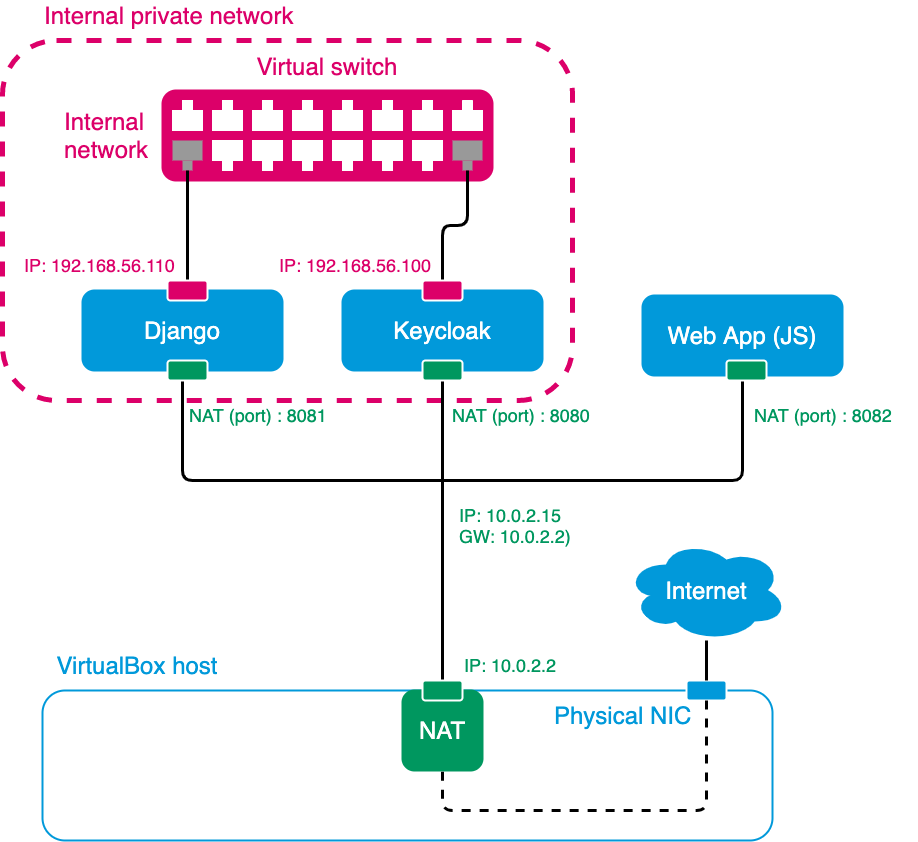
\includegraphics[width=0.7\columnwidth]{02-main/figures/keycloak_01.png}
	\captionsource{Schéma de fonctionnement du laboratoire Keycloak}{Schéma de fonctionnement du laboratoire Keycloak}{de l'auteur}
\end{figure}

\lipsum[1]
\chapter{Conclusion}
\thispagestyle{plain}
\label{chap:conclusion}
\selectlanguage{french}

%\vspace{2em}

\lipsum[1-2]

% Appendices
\appendix
% https://tex.stackexchange.com/questions/100479/label-appendix-as-appendix-i-ii-iii-rather-than-appendix-a-b-and-c
\renewcommand{\thechapter}{\Roman{chapter}}
\chapter{An appendix}
\selectlanguage{french}

\lipsum[5-8]


% -----------------------------------------------------------------------------
% Back matter
% -----------------------------------------------------------------------------
\backmatter

% Bibliography
\clearpage
\printbibliography[title={Références}, heading=bibintoc]

\clearpage
% Glossary
\printglossaries

% Page for student info and signatures
%\cleardoublepage
\chapter*{Informations sur ce travail}

\vspace{\fill}

\textbf{Informations de contact}

\begin{tabularx}{\textwidth}{N{2.5cm}X}
	Auteur:	& \AuthorFirstName \space \AuthorLastName \\
	& HES-SO Valais-Wallis \\
	E-mail: & \email{\AuthorEmail}
\end{tabularx}

\vspace{8.5cm}

\textbf{Déclaration sur l’honneur}

{\renewcommand{\arraystretch}{2}
\begin{tabularx}{\textwidth}{N{2.5cm}X}
	& Je déclare, par ce document, que j'ai effectué le travail 
	  de bachelor ci-annexé seul, sans autre aide que celles dûment 
	  signalées dans les références, et que je n'ai utilisé que les 
	  sources expressément mentionnées. Je ne donnerai aucune copie de 
	  ce rapport à un tiers sans l'autorisation conjointe du RF et du 
	  professeur chargé du suivi du travail de bachelor, à l'exception des 
	  personnes qui m'ont fourni les principales informations nécessaires 
	  à la rédaction de ce travail. \\
	Lieu, date: & \underline{\hspace{7cm}} \\ 
	Signature: & \underline{\hspace{7cm}}
\end{tabularx}
}

\vspace{\fill}

\end{document}
